\documentclass[12pt]{article}
\usepackage{amsmath,amssymb}
\setlength{\oddsidemargin}{0in}
\setlength{\evensidemargin}{0in}
\setlength{\textheight}{9in}
\setlength{\textwidth}{6.5in}
\setlength{\topmargin}{-0.5in}
\usepackage{enumitem}
\usepackage[table]{xcolor}
\usepackage{graphicx}
\usepackage{listings}
\newcommand{\Adv}{{\mathbf{Adv}}}       
\newcommand{\prp}{{\mathrm{prp}}}             
\newcommand{\calK}{{\cal K}}
\newcommand{\outputs}{{\Rightarrow}}                



% Use \textbf{Solution:}\\ to begin your solution.

%%%%%%%%%%%%%%%%%%%%%%%%%%%%%%%%%%%%%%%%%%%%%%%%%%%%%%%%%%%%%%%%%%%%%%%%%%%
\title{\bf Math 151A: Problem Set 5}
\date{ 5/19/2023}
\author{\bf Owen Jones}

\begin{document}
\maketitle


{\small \textbf{Instructions}:
\begin{itemize}
\item Due on Friday, May 19th by 1pm.
\item Late HW will not be accepted.
\item Write down all of the details and attach your code to the end of the assignment for full credit (as a PDF).  
\item If you LaTeX your solutions, you will get $5\%$ extra credit. 
\item (T) are ``pencil-and-paper'' problems and (C) means that the problem includes a computational/programming component. 
\end{itemize}}

%Add \newpage  between problems if you are using this to LaTex your solutions
\vspace{1em}

%%%%%%%%%%%%%%%%%%%%%%%%%%%%%%%%%%%%%%%%%%%%%%%%%%%%%%%%
\begin{enumerate}[label=\bfseries Problem \arabic*:]






 
%%%%%%%%%%%%%%%%%%%%%%
\item \textbf{(T) Numerical Differentiation}\\
Using the Lagrange polynomial approximation, we can show that:
\begin{align*}
f^{(4)}(x_0)= \frac{f(x_0+2h)-4f(x_0+h)+6f(x_0)-4f(x_0-h)+f(x_0-2h)}{h^4} +{O}(h^2).
\end{align*}
In this problem, you will derive this formula using the method of undetermined coefficients. Start with the following expression:
\begin{align*}
Af(x_0+2h)+Bf(x_0+h)+Cf(x_0)+Df(x_0-h)+Ef(x_0-2h).
\end{align*}
Expand each term using Taylor polynomials of degree 5 (where the sixth order term ${O}(h^6)$ is the error) and choose the coefficients in order to get an approximation to the fourth derivative. 

\textit{Hint: You will need to solve a 5-by-5 linear system. Once you have the coefficients, check that the sixth equation (corresponding to the terms involving ``$h^5\,f^{(5)}(x_0)$'') is zero. }


\vspace{1em}
 %%%%%%%%%%%%%%%%%%%%%%%%%%%%%%
\textbf{Solution:}\\
$f(x_0\pm h)=f(x_0)\pm h\cdot f'(x_0)+\frac{h^2\cdot f^{(2)}(x_0)}{2}\pm\frac{h^3\cdot f^{(3)}(x_0)}{6}+\frac{h^4\cdot f^{(4)}(x_0)}{24}\pm\frac{h^5\cdot f^{(5)}(x_0)}{120}+\frac{h^6\cdot f^{(6)}(\xi_1)}{720}$\\
$f(x_0\pm 2h)=f(x_0)\pm 2h\cdot f'(x_0)+\frac{4h^2\cdot f^{(2)}(x_0)}{2}\pm\frac{8h^3\cdot f^{(3)}(x_0)}{6}+\frac{16h^4\cdot f^{(4)}(x_0)}{24}\pm\frac{32h^5\cdot f^{(5)}(x_0)}{120}+\frac{64h^6\cdot f^{(6)}(\xi_2)}{720}$\\
$\begin{bmatrix}
    1 & 1 & 1 & 1 & 1\\
    2 & 1 & 0 & -1 & -2\\
    4 & 1 & 0 & 1 & 4\\
    8 & 1 & 0 & -1 & -8\\
    16 & 1 & 0 & 1 & 16\\
\end{bmatrix}
\times
\begin{bmatrix}
    \frac{1}{h^4}\\
    -\frac{4}{h^4}\\
    \frac{6}{h^4}\\
    -\frac{4}{h^4}\\
    \frac{1}{h^4}\\
\end{bmatrix}
=
\begin{bmatrix}
    0\\
    0\\
    0\\
    0\\
    \frac{1}{h^4}\\
\end{bmatrix}$\\
Checking to see if the coefficients for $f^{(5)}(x_0)$ sum to zero. $\frac{h\cdot f^{(5)}(x_0)}{120}(1\cdot32-4\cdot1+6\cdot0+4\cdot1-1\cdot32)=0$\\
Since they do, our error term comes from the sixth order term,\\ $\Rightarrow f^{(4)}(x_0)=\frac{f(x_0+2h)-4f(x_0+h)+6f(x_0)-4f(x_0-h)+f(x_0-2h)}{h^4} +(O)(h^2)$
\newpage
 \item \textbf{(T) Richardson's Extrapolation}\\ 
We can use lower-order formulae to generate approximations with higher accuracy. 
Consider the finite difference formula:
\begin{align}
f'(x_0)= \frac{f(x_0+h)-f(x_0)}{h}-\frac{h}{2} f^{(2)}(x_0)-\frac{h^2}{6} f^{(3)}(x_0)+O(h^3)
\end{align}
which includes more truncation terms than we used in the class.
 \begin{itemize}
\item[a)] Replacing $h$ with $2h$ in equation (1) yields the following formula:
\begin{align}
f'(x_0)= \frac{f(x_0+2h)-f(x_0)}{2h}-hf^{(2)}(x_0)-\frac{2h^2}{3} f^{(3)}(x_0)+O(h^3).
\end{align}
Using equations (1) and (2), show that :
\begin{align*}
f'(x_0)=\frac{-f(x_0+2h)+4f(x_0+h)-3f(x_0)}{2h}+\frac{h^2}{3} f^{(3)}(x_0)+O(h^3)
\end{align*}
\item[b)] Repeat the process from Part (a) with:
\begin{align*}
f'(x_0)=\frac{-f(x_0+2h)+4f(x_0+h)-3f(x_0)}{2h}+\frac{h^2}{3} f^{(3)}(x_0)+O(h^3)
\end{align*}
to show:
{ \begin{align*}
f'(x_0)=\frac{f(x_0+4h)-12f(x_0+2h)+32f(x_0+h)-21f(x_0)}{12h}+O(h^3).
\end{align*}}
 \end{itemize}


\vspace{1em}
\textbf{Solution:}
\begin{itemize}
    \item [a)] Equation (2) subtracted from $2\times$ equation (1) yields:\\
    $2(\frac{f(x_0+h)-f(x_0)}{h}-\frac{h}{2} f^{(2)}(x_0)-\frac{h^2}{6} f^{(3)}(x_0)+O(h^3))-(\frac{f(x_0+2h)-f(x_0)}{2h}-hf^{(2)}(x_0)-\frac{2h^2}{3} f^{(3)}(x_0)+O(h^3))\\
    =\frac{4f(x_0+h)-4f(x_0)}{2h}-2\frac{h}{2} f^{(2)}(x_0)-2\frac{h^2}{6} 2f^{(3)}(x_0)+2O(h^3)-(\frac{f(x_0+2h)-f(x_0)}{2h}-hf^{(2)}(x_0)-\frac{2h^2}{3} f^{(3)}(x_0)+O(h^3))\\
    =\frac{4f(x_0+h)-3f(x_0)-f(x_0+2h)}{2h}+\frac{h^2}{3} f^{(3)}(x_0)+O(h^3)$ by adding like terms.
    \item [b)] Replacing $h$ with $2h$ for the function
    \begin{align}
        f'(x_0)=\frac{-f(x_0+2h)+4f(x_0+h)-3f(x_0)}{2h}+\frac{h^2}{3} f^{(3)}(x_0)+O(h^3)    
    \end{align}
    we obtain 
    \begin{align}
        f'(x_0)=\frac{-f(x_0+4h)+4f(x_0+2h)-3f(x_0)}{4h}+\frac{4h^2}{3} f^{(3)}(x_0)+O(h^3)   
    \end{align}
    $\begin{bmatrix}
        -18 & -9\\\
        24 & 0\\
        -6 & 12\\
        0 & -3\\
    \end{bmatrix}
    \times
    \begin{bmatrix}
        \frac{4}{3}\\
        -\frac{1}{3}\\
    \end{bmatrix}
    =
    \begin{bmatrix}
        -21\\
        32\\
        -12\\
        1
    \end{bmatrix}$\\
    Subtracting $\frac{1}{3}$ equation (4) from $\frac{4}{3}$ equation (3) we obtain\\ $f'(x_0)=\frac{f(x_0+4h)-12f(x_0+2h)+32f(x_0+h)-21f(x_0)}{12h}+O(h^3)$.
\end{itemize}
%%%%%%%%%%%%%%%%%%%%%%%%%%%%%%
\newpage
 \item \textbf{(T) An Application to Parameter Estimation, Population Data}\\
Consider the logistic growth model commonly used in biology, demography, probability, sociology, {etc.}:
\begin{align*}
\frac{d}{dt}f(t) = r\,  (f(t)-f(t)^2)
\end{align*}
where $r>0$ is the constant growth rate parameter. Suppose we are given data on a population (in millions) over the last few years:
\medskip

 \begin{table}[h]
\centering
\rowcolors{1}{lightgray}{lightgray}
 \begin{tabular}{|c|c|c|c|c|c|c|}\hline
 $t$ & 2011 & 2012&  2013 & 2014 & 2015    \\ \hline
$f(t)$ &0.33000  & 0.33443  & 0.33890 & 0.34340 &  0.34792 \\ \hline
\end{tabular}
\end{table}
\medskip
\medskip

\medskip

and would like to fit the model to the data. Using the ordinary differential equation at $t=2013$ and the forward difference (2-point right-sided approximation), the central difference (3-point centered approximation), and a  5-point approximation to the derivative (check the textbook), approximate the value of $r$ (total of 3 approximations).




\vspace{1em}
\textbf{Solution:}\\
Forward $f'(t)=\frac{f(t+h)-f(t)}{h}+O(h)$ $\Rightarrow r=\frac{f(2014)-f(2013)}{f(2013)+f(2013)^2}=\frac{0.34340-0.33890}{0.33890+0.11485321}=0.009917$\\
Central $f'(t)=\frac{f(t+h)-f(t-h)}{2t}+O(h^2)$ $\Rightarrow r=\frac{f(2014)-f(2012)}{2(f(2013)+f(2013)^2)}=\frac{0.34340-0.33433}{2(0.33890+0.11485321)}=0.009994$\\
5-Point $f'(t)=\frac{1}{12h}[f(t-2h)-8f(t-h)+8f(t+h)-f(t+2h)+O(h^4)]$ $\Rightarrow r=\frac{f(2011)-8f(2012)+8f(2014)-f(2015)}{12(f(2013)+f(2013)^2)}=\frac{0.33000-8\cdot0.33443+8\cdot0.34340-0.34792}{12(0.33890+0.11485321)}=0.009888$

%%%%%%%%%%%%%%%%%%%%%%%%%%%%%%%
\newpage
 
 \item \textbf{(C) Finite Differences}\\
Write a program that computes an approximation to the first derivatives of:
\begin{description}
\item[a)] $f(x)=(x-1)^3$
\item[b)] $f(x)=(x-1)^2 \, \sin(5x)$
\end{description}
over the interval $x\in[-1,1]$ using the forward, backward, and central differences with $h=0.01$ (i.e. the grid starts at left endpoint $-1$ with spacing $h$ up to the right endpoint $1$). \textbf{Provide 6 plots} (i.e. your derivative approximation vs $x$), corresponding to each of the combinations. For credit, you must label the plots. 

\vspace{1em}
%%%%%%%%%%%%%%%%%%%%%%%%%%%%%%%%%%%
\textbf{Solution:}\\
\begin{figure}[h]
    \begin{minipage}{.5\textwidth}
        \centering
        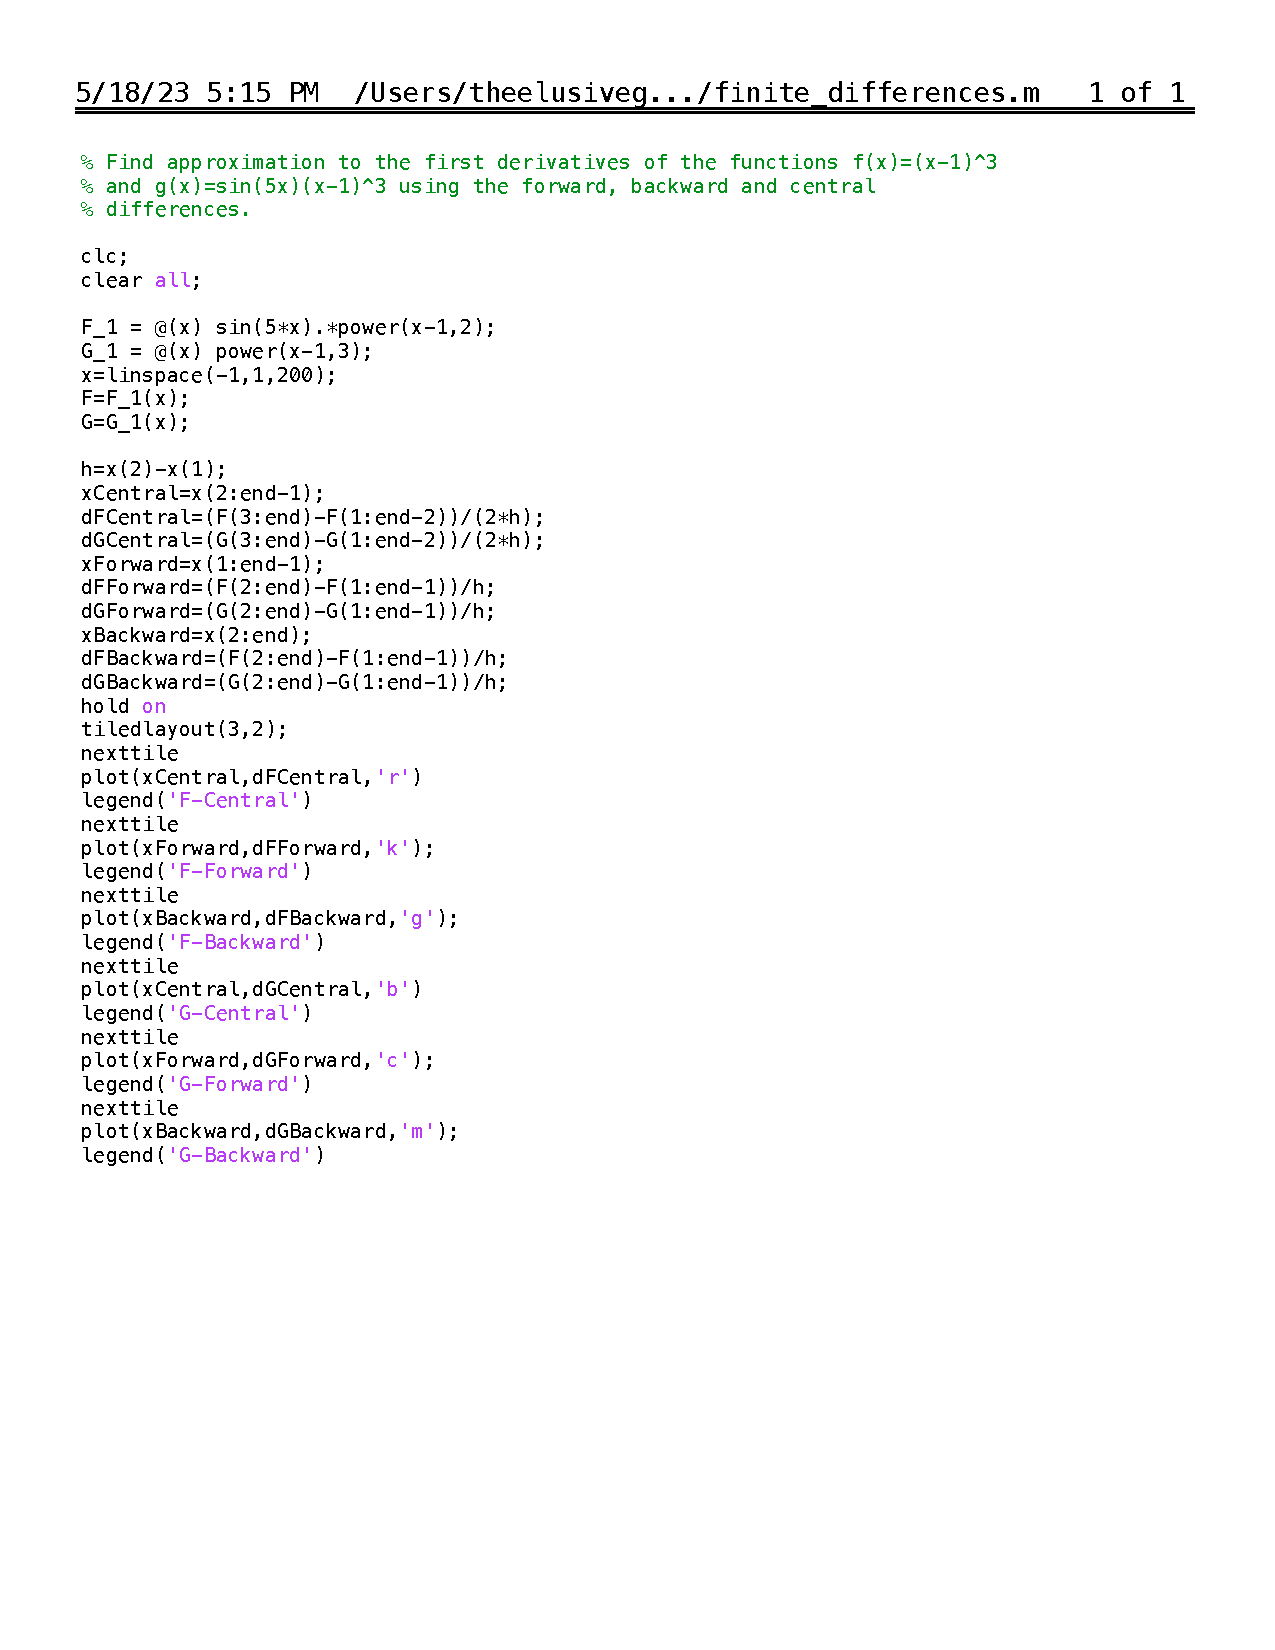
\includegraphics[width=\linewidth]{finite_difference_code.pdf} 
    \end{minipage}%
    \begin{minipage}{.5\textwidth}
        \centering
        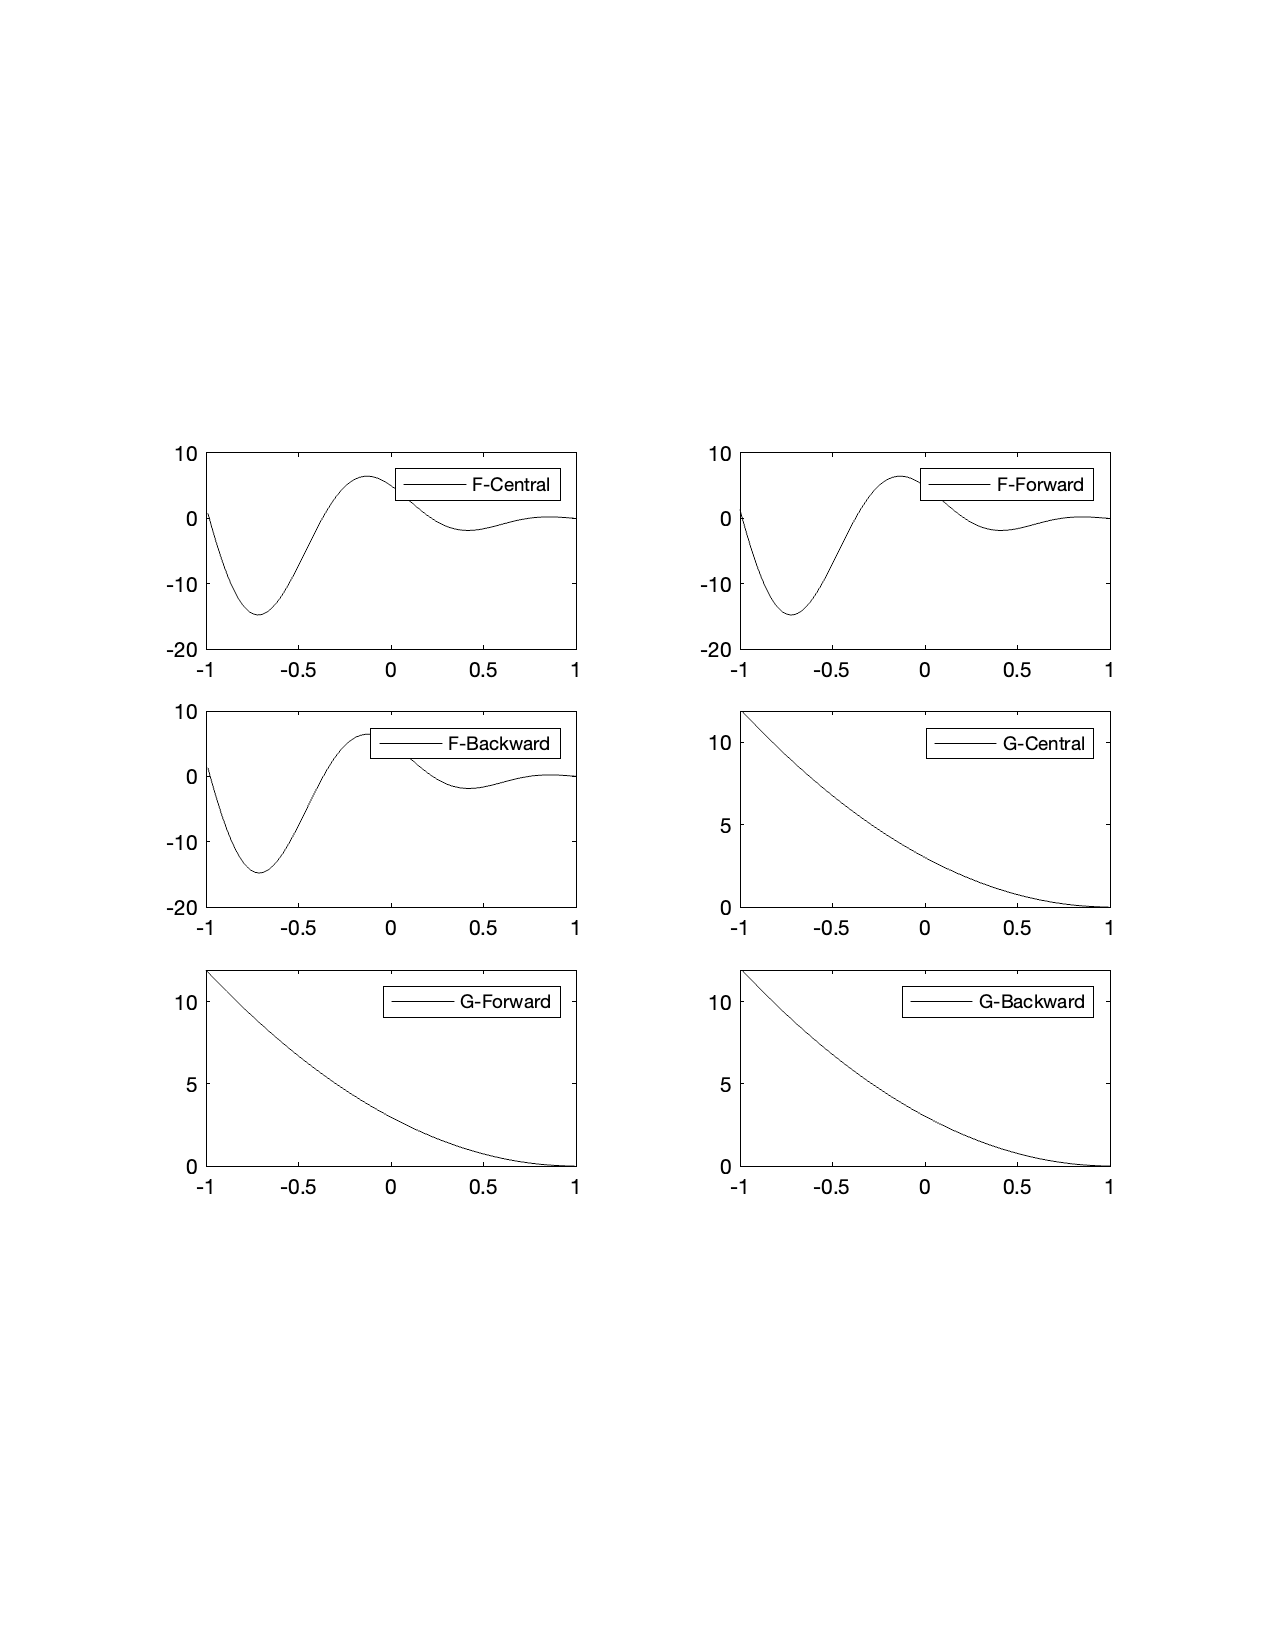
\includegraphics[width=\linewidth]{finite_difference_figure.pdf}
    \end{minipage}%         
\end{figure}



\end{enumerate}

\end{document}


